% Created by tikzDevice version 0.7.0 on 2014-09-23 11:36:12
% !TEX encoding = UTF-8 Unicode
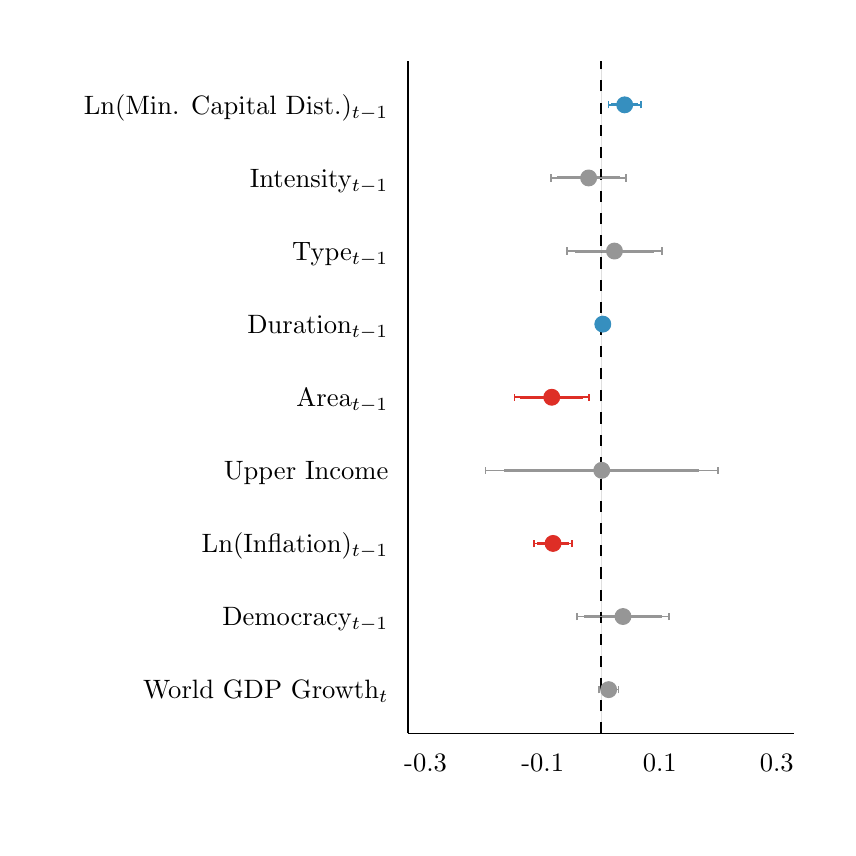
\begin{tikzpicture}[x=1pt,y=1pt]
\definecolor[named]{fillColor}{rgb}{1.00,1.00,1.00}
\path[use as bounding box,fill=fillColor,fill opacity=0.00] (0,0) rectangle (289.08,289.08);
\begin{scope}
\path[clip] (  0.00,  0.00) rectangle (289.08,289.08);
\definecolor[named]{drawColor}{rgb}{1.00,1.00,1.00}
\definecolor[named]{fillColor}{rgb}{1.00,1.00,1.00}

\path[draw=drawColor,line width= 0.6pt,line join=round,line cap=round,fill=fillColor] ( -0.00,  0.00) rectangle (289.08,289.08);
\end{scope}
\begin{scope}
\path[clip] (137.46, 34.03) rectangle (277.03,277.03);
\definecolor[named]{fillColor}{rgb}{1.00,1.00,1.00}

\path[fill=fillColor] (137.46, 34.03) rectangle (277.03,277.03);
\definecolor[named]{drawColor}{rgb}{0.59,0.59,0.59}
\definecolor[named]{fillColor}{rgb}{0.59,0.59,0.59}

\path[draw=drawColor,draw opacity=0.30,line width= 0.3pt,line join=round,fill=fillColor,fill opacity=0.30] (206.43, 49.88) -- (213.45, 49.88);

\path[draw=drawColor,draw opacity=0.30,line width= 0.3pt,line join=round,fill=fillColor,fill opacity=0.30] (198.47, 76.30) -- (231.75, 76.30);
\definecolor[named]{drawColor}{rgb}{0.87,0.18,0.15}
\definecolor[named]{fillColor}{rgb}{0.87,0.18,0.15}

\path[draw=drawColor,draw opacity=0.30,line width= 0.3pt,line join=round,fill=fillColor,fill opacity=0.30] (183.03,102.71) -- (196.68,102.71);
\definecolor[named]{drawColor}{rgb}{0.59,0.59,0.59}
\definecolor[named]{fillColor}{rgb}{0.59,0.59,0.59}

\path[draw=drawColor,draw opacity=0.30,line width= 0.3pt,line join=round,fill=fillColor,fill opacity=0.30] (165.42,129.12) -- (249.46,129.12);
\definecolor[named]{drawColor}{rgb}{0.87,0.18,0.15}
\definecolor[named]{fillColor}{rgb}{0.87,0.18,0.15}

\path[draw=drawColor,draw opacity=0.30,line width= 0.3pt,line join=round,fill=fillColor,fill opacity=0.30] (175.86,155.53) -- (202.88,155.53);
\definecolor[named]{drawColor}{rgb}{0.21,0.56,0.75}
\definecolor[named]{fillColor}{rgb}{0.21,0.56,0.75}

\path[draw=drawColor,draw opacity=0.30,line width= 0.3pt,line join=round,fill=fillColor,fill opacity=0.30] (207.28,181.95) -- (208.37,181.95);
\definecolor[named]{drawColor}{rgb}{0.59,0.59,0.59}
\definecolor[named]{fillColor}{rgb}{0.59,0.59,0.59}

\path[draw=drawColor,draw opacity=0.30,line width= 0.3pt,line join=round,fill=fillColor,fill opacity=0.30] (194.89,208.36) -- (229.18,208.36);

\path[draw=drawColor,draw opacity=0.30,line width= 0.3pt,line join=round,fill=fillColor,fill opacity=0.30] (189.15,234.77) -- (216.25,234.77);
\definecolor[named]{drawColor}{rgb}{0.21,0.56,0.75}
\definecolor[named]{fillColor}{rgb}{0.21,0.56,0.75}

\path[draw=drawColor,draw opacity=0.30,line width= 0.3pt,line join=round,fill=fillColor,fill opacity=0.30] (209.85,261.19) -- (221.60,261.19);
\definecolor[named]{drawColor}{rgb}{0.59,0.59,0.59}
\definecolor[named]{fillColor}{rgb}{0.59,0.59,0.59}

\path[draw=drawColor,line width= 1.1pt,line join=round,fill=fillColor] (206.99, 49.88) -- (212.88, 49.88);

\path[draw=drawColor,line width= 1.1pt,line join=round,fill=fillColor] (201.15, 76.30) -- (229.08, 76.30);
\definecolor[named]{drawColor}{rgb}{0.87,0.18,0.15}
\definecolor[named]{fillColor}{rgb}{0.87,0.18,0.15}

\path[draw=drawColor,line width= 1.1pt,line join=round,fill=fillColor] (184.13,102.71) -- (195.58,102.71);
\definecolor[named]{drawColor}{rgb}{0.59,0.59,0.59}
\definecolor[named]{fillColor}{rgb}{0.59,0.59,0.59}

\path[draw=drawColor,line width= 1.1pt,line join=round,fill=fillColor] (172.18,129.12) -- (242.71,129.12);
\definecolor[named]{drawColor}{rgb}{0.87,0.18,0.15}
\definecolor[named]{fillColor}{rgb}{0.87,0.18,0.15}

\path[draw=drawColor,line width= 1.1pt,line join=round,fill=fillColor] (178.04,155.53) -- (200.70,155.53);
\definecolor[named]{drawColor}{rgb}{0.21,0.56,0.75}
\definecolor[named]{fillColor}{rgb}{0.21,0.56,0.75}

\path[draw=drawColor,line width= 1.1pt,line join=round,fill=fillColor] (207.37,181.95) -- (208.28,181.95);
\definecolor[named]{drawColor}{rgb}{0.59,0.59,0.59}
\definecolor[named]{fillColor}{rgb}{0.59,0.59,0.59}

\path[draw=drawColor,line width= 1.1pt,line join=round,fill=fillColor] (197.65,208.36) -- (226.42,208.36);

\path[draw=drawColor,line width= 1.1pt,line join=round,fill=fillColor] (191.33,234.77) -- (214.07,234.77);
\definecolor[named]{drawColor}{rgb}{0.21,0.56,0.75}
\definecolor[named]{fillColor}{rgb}{0.21,0.56,0.75}

\path[draw=drawColor,line width= 1.1pt,line join=round,fill=fillColor] (210.79,261.19) -- (220.66,261.19);
\definecolor[named]{drawColor}{rgb}{0.00,0.00,0.00}
\definecolor[named]{fillColor}{rgb}{0.00,0.00,0.00}

\path[draw=drawColor,line width= 0.6pt,dash pattern=on 4pt off 4pt ,line join=round,fill=fillColor] (207.25, 34.03) -- (207.25,277.03);
\definecolor[named]{drawColor}{rgb}{0.21,0.56,0.75}
\definecolor[named]{fillColor}{rgb}{0.21,0.56,0.75}

\path[draw=drawColor,line width= 0.4pt,line join=round,line cap=round,fill=fillColor] (215.73,261.19) circle (  2.85);
\definecolor[named]{drawColor}{rgb}{0.59,0.59,0.59}
\definecolor[named]{fillColor}{rgb}{0.59,0.59,0.59}

\path[draw=drawColor,line width= 0.4pt,line join=round,line cap=round,fill=fillColor] (202.70,234.77) circle (  2.85);

\path[draw=drawColor,line width= 0.4pt,line join=round,line cap=round,fill=fillColor] (212.04,208.36) circle (  2.85);
\definecolor[named]{drawColor}{rgb}{0.21,0.56,0.75}
\definecolor[named]{fillColor}{rgb}{0.21,0.56,0.75}

\path[draw=drawColor,line width= 0.4pt,line join=round,line cap=round,fill=fillColor] (207.82,181.95) circle (  2.85);
\definecolor[named]{drawColor}{rgb}{0.87,0.18,0.15}
\definecolor[named]{fillColor}{rgb}{0.87,0.18,0.15}

\path[draw=drawColor,line width= 0.4pt,line join=round,line cap=round,fill=fillColor] (189.37,155.53) circle (  2.85);
\definecolor[named]{drawColor}{rgb}{0.59,0.59,0.59}
\definecolor[named]{fillColor}{rgb}{0.59,0.59,0.59}

\path[draw=drawColor,line width= 0.4pt,line join=round,line cap=round,fill=fillColor] (207.44,129.12) circle (  2.85);
\definecolor[named]{drawColor}{rgb}{0.87,0.18,0.15}
\definecolor[named]{fillColor}{rgb}{0.87,0.18,0.15}

\path[draw=drawColor,line width= 0.4pt,line join=round,line cap=round,fill=fillColor] (189.85,102.71) circle (  2.85);
\definecolor[named]{drawColor}{rgb}{0.59,0.59,0.59}
\definecolor[named]{fillColor}{rgb}{0.59,0.59,0.59}

\path[draw=drawColor,line width= 0.4pt,line join=round,line cap=round,fill=fillColor] (215.11, 76.30) circle (  2.85);

\path[draw=drawColor,line width= 0.4pt,line join=round,line cap=round,fill=fillColor] (209.94, 49.88) circle (  2.85);

\path[draw=drawColor,line width= 0.6pt,line join=round] (213.45, 48.56) --
	(213.45, 51.20);

\path[draw=drawColor,line width= 0.6pt,line join=round] (213.45, 49.88) --
	(206.43, 49.88);

\path[draw=drawColor,line width= 0.6pt,line join=round] (206.43, 48.56) --
	(206.43, 51.20);

\path[draw=drawColor,line width= 0.6pt,line join=round] (231.75, 74.97) --
	(231.75, 77.62);

\path[draw=drawColor,line width= 0.6pt,line join=round] (231.75, 76.30) --
	(198.47, 76.30);

\path[draw=drawColor,line width= 0.6pt,line join=round] (198.47, 74.97) --
	(198.47, 77.62);
\definecolor[named]{drawColor}{rgb}{0.87,0.18,0.15}

\path[draw=drawColor,line width= 0.6pt,line join=round] (196.68,101.39) --
	(196.68,104.03);

\path[draw=drawColor,line width= 0.6pt,line join=round] (196.68,102.71) --
	(183.03,102.71);

\path[draw=drawColor,line width= 0.6pt,line join=round] (183.03,101.39) --
	(183.03,104.03);
\definecolor[named]{drawColor}{rgb}{0.59,0.59,0.59}

\path[draw=drawColor,line width= 0.6pt,line join=round] (249.46,127.80) --
	(249.46,130.44);

\path[draw=drawColor,line width= 0.6pt,line join=round] (249.46,129.12) --
	(165.42,129.12);

\path[draw=drawColor,line width= 0.6pt,line join=round] (165.42,127.80) --
	(165.42,130.44);
\definecolor[named]{drawColor}{rgb}{0.87,0.18,0.15}

\path[draw=drawColor,line width= 0.6pt,line join=round] (202.88,154.21) --
	(202.88,156.86);

\path[draw=drawColor,line width= 0.6pt,line join=round] (202.88,155.53) --
	(175.86,155.53);

\path[draw=drawColor,line width= 0.6pt,line join=round] (175.86,154.21) --
	(175.86,156.86);
\definecolor[named]{drawColor}{rgb}{0.21,0.56,0.75}

\path[draw=drawColor,line width= 0.6pt,line join=round] (208.37,180.63) --
	(208.37,183.27);

\path[draw=drawColor,line width= 0.6pt,line join=round] (208.37,181.95) --
	(207.28,181.95);

\path[draw=drawColor,line width= 0.6pt,line join=round] (207.28,180.63) --
	(207.28,183.27);
\definecolor[named]{drawColor}{rgb}{0.59,0.59,0.59}

\path[draw=drawColor,line width= 0.6pt,line join=round] (229.18,207.04) --
	(229.18,209.68);

\path[draw=drawColor,line width= 0.6pt,line join=round] (229.18,208.36) --
	(194.89,208.36);

\path[draw=drawColor,line width= 0.6pt,line join=round] (194.89,207.04) --
	(194.89,209.68);

\path[draw=drawColor,line width= 0.6pt,line join=round] (216.25,233.45) --
	(216.25,236.09);

\path[draw=drawColor,line width= 0.6pt,line join=round] (216.25,234.77) --
	(189.15,234.77);

\path[draw=drawColor,line width= 0.6pt,line join=round] (189.15,233.45) --
	(189.15,236.09);
\definecolor[named]{drawColor}{rgb}{0.21,0.56,0.75}

\path[draw=drawColor,line width= 0.6pt,line join=round] (221.60,259.87) --
	(221.60,262.51);

\path[draw=drawColor,line width= 0.6pt,line join=round] (221.60,261.19) --
	(209.85,261.19);

\path[draw=drawColor,line width= 0.6pt,line join=round] (209.85,259.87) --
	(209.85,262.51);
\end{scope}
\begin{scope}
\path[clip] (  0.00,  0.00) rectangle (289.08,289.08);
\definecolor[named]{drawColor}{rgb}{0.00,0.00,0.00}

\path[draw=drawColor,line width= 0.6pt,line join=round] (137.46, 34.03) --
	(137.46,277.03);
\end{scope}
\begin{scope}
\path[clip] (  0.00,  0.00) rectangle (289.08,289.08);
\definecolor[named]{drawColor}{rgb}{0.00,0.00,0.00}

\node[text=drawColor,anchor=base east,inner sep=0pt, outer sep=0pt, scale=  0.96] at (130.35, 46.58) {World GDP Growth$_{t}$};

\node[text=drawColor,anchor=base east,inner sep=0pt, outer sep=0pt, scale=  0.96] at (130.35, 72.99) {Democracy$_{t-1}$};

\node[text=drawColor,anchor=base east,inner sep=0pt, outer sep=0pt, scale=  0.96] at (130.35, 99.40) {Ln(Inflation)$_{t-1}$};

\node[text=drawColor,anchor=base east,inner sep=0pt, outer sep=0pt, scale=  0.96] at (130.35,125.82) {Upper Income};

\node[text=drawColor,anchor=base east,inner sep=0pt, outer sep=0pt, scale=  0.96] at (130.35,152.23) {Area$_{t-1}$};

\node[text=drawColor,anchor=base east,inner sep=0pt, outer sep=0pt, scale=  0.96] at (130.35,178.64) {Duration$_{t-1}$};

\node[text=drawColor,anchor=base east,inner sep=0pt, outer sep=0pt, scale=  0.96] at (130.35,205.06) {Type$_{t-1}$};

\node[text=drawColor,anchor=base east,inner sep=0pt, outer sep=0pt, scale=  0.96] at (130.35,231.47) {Intensity$_{t-1}$};

\node[text=drawColor,anchor=base east,inner sep=0pt, outer sep=0pt, scale=  0.96] at (130.35,257.88) {Ln(Min. Capital Dist.)$_{t-1}$};
\end{scope}
\begin{scope}
\path[clip] (  0.00,  0.00) rectangle (289.08,289.08);
\definecolor[named]{drawColor}{rgb}{0.00,0.00,0.00}

\path[draw=drawColor,line width= 0.6pt,line join=round] (137.46, 34.03) --
	(277.03, 34.03);
\end{scope}
\begin{scope}
\path[clip] (  0.00,  0.00) rectangle (289.08,289.08);
\definecolor[named]{drawColor}{rgb}{0.00,0.00,0.00}

\node[text=drawColor,anchor=base,inner sep=0pt, outer sep=0pt, scale=  0.96] at (143.80, 20.31) {-0.3};

\node[text=drawColor,anchor=base,inner sep=0pt, outer sep=0pt, scale=  0.96] at (186.10, 20.31) {-0.1};

\node[text=drawColor,anchor=base,inner sep=0pt, outer sep=0pt, scale=  0.96] at (228.40, 20.31) {0.1};

\node[text=drawColor,anchor=base,inner sep=0pt, outer sep=0pt, scale=  0.96] at (270.69, 20.31) {0.3};
\end{scope}
\end{tikzpicture}
